% Hlavička
\documentclass{article}

% Preambule - použité balíčky
\usepackage[czech]{babel}		% Čeština (nadpisy, dělení slov, speciální akcenty, jako například ď)
\usepackage{amsmath,amsfonts}	% Matematické symboly a prostředí
\usepackage[utf8]{inputenc}		% Kódování vstupního textu (jinak pouhé ASCII)
\usepackage[unicode]{hyperref}	% Rovnice elegantně odkazy
\usepackage{graphicx}			% Vkládání obrázků
\usepackage{indentfirst}		% České odsazení prvního odstavce 
						
% Tělo dokumentu
\begin{document}
\section{Dvojité kyvadlo}
    \begin{center}
        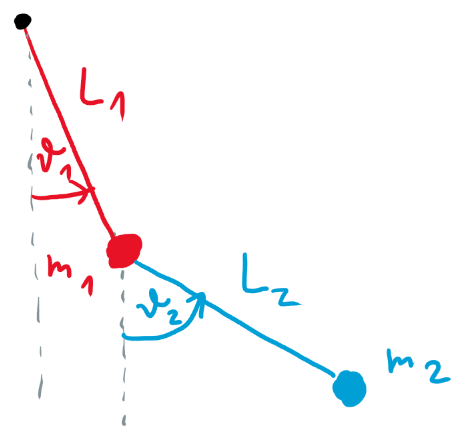
\includegraphics[width=0.495\linewidth]{dvojkyvadlo.png}
    \end{center}
    \subsection{Energie}
    Kinetická a potenciální energie pro dvojité kyvadlo parametrizované dle obrázku se dají vyjádřit následovně:
    \begin{align}
        T &= \frac{1}{2} m L_1^2 \dot{\theta}_1^2 + \frac{1}{2} m_2 L_2^2 \dot{\theta}_2^2 + m_{2} L_1 L_2 \dot{\theta}_1 \dot{\theta}_2 \cos\Delta\theta, \\
        V &= m g L_1 (1 - \cos \theta_1) + m_2 g L_2 (1 - \cos \theta_2),
    \end{align}
    kde $m=m_1+m_2$ je součet hmotností obou kyvadel, $L_1$ a $L_2$ jejich délky, $\theta_1$ a $\theta_2$ jsou úhly vychýlení od svislé polohy, $\Delta\theta=\theta_{1}-\theta_{2}$ jejich rozdíl, $\omega_{1}=\dot{\theta}_1$ a $\omega_{2}=\dot{\theta}_2$ jsou úhlové rychlosti a $g$ je tíhové zrychlení.
    Při této parametrizaci je celková energie $E=T+V$ nulová, pokud je kyvadlo v klidu ve svislé poloze, a je vždy kladná, pokud se kyvadlo pohybuje.

    Hmotnosti závěsů se zanedbávají.

    \subsection{Pohybové rovnice}
    Pohybové rovnice pro dvojité kyvadlo lze zapsat ve tvaru
    \begin{subequations}
        \begin{align}
            \ddot{\theta}_1 &= \frac{-\sin{\Delta\theta}\left(m_{2}L_1\dot{\theta}_1^2\cos{\Delta\theta}+m_{2}L_{2}\dot{\theta}_2^2\right)
                -g\left(m\sin{\theta_1}-m_2\sin{\theta_{2}}\cos{\Delta\theta}\right)}{2L_{1}A},\\
            \ddot{\theta}_2 &= \frac{+\sin{\Delta\theta}\left(m_{2}L_2\dot{\theta}_2^2\cos{\Delta\theta}+m L_{1}\dot{\theta}_1^2\right)
                -g\left(m\sin{\theta_2}-m\sin{\theta_{1}}\cos{\Delta\theta}\right)}{2L_{2}A},
        \end{align}
        \label{eq:motion}            
    \end{subequations}
    kde $A=m_{1}+m_{2}\sin^2{\Delta\theta}$.
    Odvození těchto rovnic je celkem složité, využívá se formalizmu Lagrangeových rovnic druhého druhu, který se naučíte až v druhém ročníku v předmětu Teoretická mechanika.
    Konkrétní postup je popsán například v \cite{DP}.
    
    Jednoduchý Verletův algoritmus není pro řešení těchto rovnic vhodný, proto\-že soustava není ve tvaru 
    \begin{equation}
        \ddot{\boldsymbol{\theta}}={\boldsymbol{f}}(\boldsymbol{\theta})
    \end{equation}
    kde $\boldsymbol{\theta}=(\theta_1,\theta_2)$ (pravá strana závisí i na derivacích $\dot{\boldsymbol{\theta}}$).
    K řešení Vám doporučuji použít Eulerovu metodu 2. řádu nebo Runge-Kuttovu metodu 4. řádu, které jsme probírali na cvičení.
    Soustavu dvou rovnic druhého řádu~\eqref{eq:motion} převedete na soustavu čtyř rovnic prvního řádu využitím pomocných funkcí $\omega_{1,2}=\dot{\theta}_{1,2}$.

    \subsection{Zápočet}
    Pro zápočet naprogramujte:
    \begin{enumerate}
        \item Řešení pohybových rovnic~\eqref{eq:motion}.
            Kontrolou by Vám mělo být, že celková energie $E$ se bude v průběhu času zachovávat.

        \item Generování přesných počátečních podmínek.
            Doporučuji nagenerovat ná\-hod\-ně $\theta_1$ a $\theta_2$ z intervalu $(-\pi,\pi)$ tak, jak již počítáte.
            Dále využijte toho, že kinetická energie nemůže být záporná.
            Opakujte tedy generování úhlů do té doby, než $V(\theta_{1},\theta_{2})<E$.
            Poté odhadněte interval pro $\omega_{1}=\theta_{1}$ řešením nerovnice 
            \begin{equation}
                T(\omega_{1},\omega_{2}=0)\leq E-V(\theta_{1},\theta_{2})
            \end{equation}
            pro $\omega_{1}$, čímž získáte interval pro $\omega_{1}$, ze kterého $\omega_{1}$ nagenerujete náhodně.
            Nakonec vyřešíte rovnici 
            \begin{equation}
                T(\omega_{1},\omega_{2})=E-V(\theta_{1},\theta_{2})
            \end{equation}
            pro $\omega_{2}$.

        \item Vykreslení animace pohybu kyvadla.
    \end{enumerate}
    Poincarého řez programovat nemusíte.

    \begin{thebibliography}{9}
        \bibitem{DP} \url{https://physicspython.wordpress.com/2019/04/26/double-pendulum-part-2/}
    \end{thebibliography}

\end{document}
